\documentclass[12pt,oneside]{uhthesis}
\usepackage{subfigure}
\usepackage[ruled,lined,linesnumbered,titlenumbered,algochapter,spanish,onelanguage]{algorithm2e}
\usepackage{amsmath}
\usepackage{amssymb}
\usepackage{amsbsy}
\usepackage{caption,booktabs}
\captionsetup{ justification = centering }
%\usepackage{mathpazo}
\usepackage{float}
\setlength{\marginparwidth}{2cm}
\usepackage{todonotes}
\usepackage{listings}
\usepackage{xcolor}
\usepackage{multicol}
\usepackage{graphicx}
\usepackage{newclude}
\usepackage{hyperref}

\floatstyle{plaintop}
\restylefloat{table}
\addbibresource{Bibliography.bib}
% \setlength{\parskip}{\baselineskip}%
\renewcommand{\tablename}{Tabla}
\renewcommand{\listalgorithmcfname}{Índice de Algoritmos}
%\dontprintsemicolon
\SetAlgoNoEnd

\definecolor{codegreen}{rgb}{0,0.6,0}
\definecolor{codegray}{rgb}{0.5,0.5,0.5}
\definecolor{codepurple}{rgb}{0.58,0,0.82}
\definecolor{backcolour}{rgb}{0.95,0.95,0.92}

\lstdefinestyle{mystyle}{
    backgroundcolor=\color{backcolour},   
    commentstyle=\color{codegreen},
    keywordstyle=\color{purple},
    numberstyle=\tiny\color{codegray},
    stringstyle=\color{codepurple},
    basicstyle=\ttfamily\footnotesize,
    breakatwhitespace=false,         
    breaklines=true,                 
    captionpos=b,                    
    keepspaces=true,                 
    numbers=left,                    
    numbersep=5pt,                  
    showspaces=false,                
    showstringspaces=false,
    showtabs=false,                  
    tabsize=4
}

\lstset{style=mystyle}

\title{Modelación de la Especialización Hemisférica para Frecuencias Espaciales a través de Campos Receptivos Poblacionales}
\author{\\\vspace{0.25cm}Mari\'e del Valle Reyes}
\advisor{\\\vspace{0.25cm}Dr. Mitchell Valdes Sosa\\\vspace{0.2cm}MSc. Ania Mesa Rodr\'iguez}
\degree{Licenciado en Ciencia de la Computación}
\faculty{Facultad de Matemática y Computación}
\date{
\includegraphics[scale=0.3]{Graphics/qrcode-generado}\\\vspace{0.25cm}2024}}
\logo{Graphics/uhlogo}
\makenomenclature

\renewcommand{\vec}[1]{\boldsymbol{#1}}
\newcommand{\diff}[1]{\ensuremath{\mathrm{d}#1}}
\newcommand{\me}[1]{\mathrm{e}^{#1}}
\newcommand{\pf}{\mathfrak{p}}
\newcommand{\qf}{\mathfrak{q}}
%\newcommand{\kf}{\mathfrak{k}}
\newcommand{\kt}{\mathtt{k}}
\newcommand{\mf}{\mathfrak{m}}
\newcommand{\hf}{\mathfrak{h}}
\newcommand{\fac}{\mathrm{fac}}
\newcommand{\maxx}[1]{\max\left\{ #1 \right\} }
\newcommand{\minn}[1]{\min\left\{ #1 \right\} }
\newcommand{\lldpcf}{1.25}
\newcommand{\nnorm}[1]{\left\lvert #1 \right\rvert }
\renewcommand{\lstlistingname}{Ejemplo de código}
\renewcommand{\lstlistlistingname}{Ejemplos de código}

\begin{document}

\frontmatter
\maketitle

\begin{dedication}
    \textbf{\textit{A mi familia, mi br\'ujula en la traves\'ia\\ y mi refugio en la tormenta.}}
\end{dedication}
\begin{acknowledgements}
    Agradecimientos
\end{acknowledgements}
\begin{opinion}
    La división de funciones entre los dos hemisferios cerebrales ha sido uno de los temas más intensamente estudiados en las neurociencias desde hace dos siglos, en particular en los procesos visuales. Esto ha generado un volumen valioso de datos psicológicos y clínicos. Con el desarrollo de los métodos modernos de neuroimágenes, se ha obtenido aún más información. Sin embargo, no han generado modelos cuantitativos que puedan explicar cómo se diferencian los dos hemisferios. Hay más datos que teoría sólida. El lenguaje natural para formular modelos apropiados parece estar en el terreno de redes neurales convolucionales profundas, las cuales deben su reciente éxito práctico en diversos campos tecnológicos en su imitación al sistema visual humano. El desarrollo de la modelación de los campos receptivos poblacionales a partir de datos de resonancia magnética funcional abre el camino a modelos de redes neurales convolucionales m\'as realistas.  La tesis de Mari\'e del Valle Reyes sería un primer paso en examinar con campos receptivos poblacionales la lateralización hemisférica de los procesos visuales.
    
    Mari\'e del Valle Reyes es una alumna muy destacada, trabajando con entusiasmo de forma incansable. La estudiante ha demostrado una integración valiosa de habilidades en matemáticas aplicadas a la neurociencia en su tesis de diploma. Ha combinado una capacidad de programación en varios lenguajes (como Python, R, y Matlab) con el aprendizaje rápido de modelos estadísticos avanzados, y el aprendizaje de temas de neurociencias. Su capacidad para traducir conceptos matemáticos complejos en herramientas aplicables a la comprensión de procesos neurales muestra un enfoque interdisciplinario y original. Se han obtenido resultados importantes ya casi maduros para publicar en poco tiempo gracias a su tenacidad y entrega al trabajo. Su investigación es una contribución prometedora en la convergencia de las matemáticas y las neurociencias. Ha sido un gusto trabajar con ella.
\end{opinion}
\begin{resumen}
	El estudio analiza cómo los hemisferios cerebrales se especializan en procesar frecuencias espaciales de est\'imulos visuales, mediante modelos de campos receptivos poblacionales y modelos lineales mixtos. Se enfoca en el período preferido de los vértices corticales en diferentes áreas visuales, explorando su relación con la excentricidad visual y su influencia en la lateralización hemisférica. Los resultados revelan que el hemisferio derecho tiende a procesar frecuencias más bajas que el hemisferio izquierdo en áreas visuales superiores, aunque esta tendencia no se observa en áreas visuales primarias.  Este trabajo favorece la comprensión de cómo se procesa y representa la información visual, contribuyendo significativamente al conocimiento sobre la especialización funcional de los hemisferios en distintos niveles de procesamiento visual.
\end{resumen}

\begin{abstract}
	The study examines how the cerebral hemispheres specialize in processing spatial frequencies of visual stimuli using models of population receptive fields and mixed linear models. It focuses on the preferred period of cortical vertices in different visual areas, exploring its relationship with visual eccentricity and its influence on hemispheric lateralization. The results reveal that the right hemisphere tends to process lower frequencies than the left hemisphere in higher visual areas, although this trend is not observed in primary visual areas. This work enhances our understanding of how visual information is processed and represented, making a significant contribution to our knowledge of the functional specialization of the hemispheres at different levels of visual processing.
\end{abstract}
\tableofcontents
\listoffigures
% \listoftables
% \listofalgorithms
\lstlistoflistings

\mainmatter


\chapter*{Introducción}\label{chapter:introduction}
\addcontentsline{toc}{chapter}{Introducción}
El cerebro humano se concibe como un sistema complejo que controla y regula la mayoría de las funciones del cuerpo y de la mente. Este \'organo desempeña un papel esencial en la percepción y el procesamiento de la información, debido a que es el encargado de recibir, interpretar y responder a los estímulos del entorno, lo cual permite a los individuos interactuar de manera efectiva con su mundo. La percepción implica la interpretación y organización de los estímulos sensoriales para formar una representación consciente de la realidad. El cerebro procesa la información visual, auditiva, táctil y otras modalidades sensoriales, integrándola para construir una experiencia coherente y significativa del entorno circundante.

Los dos hemisferios cerebrales desempeñan papeles notablemente diferentes en la percepción visual a pesar de su estrecha interacción, evidenciándose una lateralización hemisférica. Esta asimetría funcional se ha documentado exhaustivamente para procesar aspectos globales y locales de estímulos visuales \cite{flevaris_spatial_2016}, donde el hemisferio derecho muestra un sesgo global y el hemisferio izquierdo muestra una preferencia local. Estos sesgos para los niveles local/global se han establecido a través de métodos psicofísicos \cite{brederoo_hemispheric_2017, brederoo_reproducibility_2019} y electrofisiológicos \cite{flevaris_attending_2014, iglesias-fuster_asynchronous_2015, jiang_neural_2005}.

El sesgo global/local de los hemisferios derecho/izquierdo podría explicarse en términos de las frecuencias espaciales (SF) asociadas con diferentes niveles de un estímulo visual. Las frecuencias espaciales describen cómo varía la información visual en términos de patrones de luz y sombra en una escena. Estos patrones pueden involucrar detalles finos o cambios suaves en la luminosidad. En el contexto visual, las SF más bajas se asocian comúnmente con aspectos globales, mientras que las SF más altas se asocian con aspectos locales \cite{flevaris_spatial_2016}. En apoyo a esta idea, varios estudios han revelado un sesgo hacia SF más bajas en el hemisferio derecho y SF más altas en el hemisferio izquierdo \cite{flevaris_spatial_2016}. Esto implica que el hemisferio derecho puede ser más eficiente en procesar información visual relacionada con la configuración global de un estímulo, mientras que el hemisferio izquierdo podría destacarse en detalles locales más finos. Además, se han encontrado vínculos entre la selección atencional global/local y las frecuencias espaciales de los est\'imulos \cite{flevaris_spatial_2016}. Sin embargo, cualquier teoría basada en estas consideraciones debe tener en cuenta el hecho de que los mismos aspectos de un estímulo visual pueden ser globales en un contexto y locales en otro (por ejemplo, un árbol es global en relación con una hoja pero local en relación con un bosque). El papel de cualquier SF no es fijo sino que depende del contexto.	

Una posible forma de evaluar y medir la lateralización hemisférica se presenta a través de la medición de los campos receptivos de la población (pRF) mediante resonancia magnética funcional (fMRI) \cite{dumoulin_population_2008, kay_principles_2018} . Los pRF constituyen modelos cuantitativos que describen la respuesta combinada de las neuronas dentro de un vóxel de fMRI (vértice cortical). Estos modelos suelen estimar la posición y el tamaño de la sección del campo visual que afecta a un vóxel específico \cite{wandell_computational_2015}. La medición de respuestas de frecuencia espacial (SF) en los pRF también se ha convertido en un enfoque relevante, especialmente en áreas visuales tempranas (área visual primaria, V2, V3), ofreciendo perspectivas adicionales sobre la sintonización de SF en relación con el tamaño del pRF. Investigaciones recientes \cite{aghajari_population_2020, broderick_mapping_2022} han demostrado que la sintonización de la frecuencia espacial de un pRF tiende a disminuir a medida que aumenta su tamaño, lo que sugiere una posible relación entre la lateralización hemisférica y las características de procesamiento de la información visual en el cerebro. Estas observaciones brindan una valiosa perspectiva para comprender cómo la lateralización hemisférica puede estar vinculada a las propiedades de los campos receptivos de la población.

La investigación sobre las propiedades de los pRF en funci\'on del campo visual, se ha focalizado principalmente en las diferencias entre los cuadrantes superior e inferior en la corteza visual primaria (V1), donde no se han observado diferencias significativas entre los cuadrantes derecho e izquierdo. Un estudio encontró tamaños de pRF ligeramente más pequeños en el cuadrante izquierdo en comparación con los cuadrantes horizontales derechos de las \'areas visuales V2 y V3 y, nuevamente, no hubo diferencias en V1 \cite{silva_radial_2018}. Esta observación sugiere que la lateralidad de las propiedades de los pRF en áreas visuales intermedias y superiores no se ha estudiado exhaustivamente. La dificultad para identificar sitios homólogos entre hemisferios en estas regiones, donde los mapas retinotópicos son menos definidos, puede contribuir a la falta de investigación detallada en estas áreas.

Existen varias bases de datos p\'ublicas de pRF \cite{benson_bayesian_2018,himmelberg_cross-dataset_2021}, que cubren amplias extensiones de la corteza cerebral, lo que hace posible la prueba de la lateralidad de las propiedades de pRF en \'areas visuales de orden intermedio o superior. Para examinar las diferencias derecha/izquierda en el tamaño del pRF, se pueden utilizar dos estrategias denominadas aquí \textbf{anatómicas} y \textbf{homotópicas}. El objetivo es comparar sitios corticales homólogos, pero como se mencionó anteriormente, definir "homólogo" presenta dificultades, especialmente para áreas de orden superior con respuesta visual.

La estrategia anatómica mide las diferencias en las propiedades de pRF en un espacio donde las superficies corticales son aproximadamente simétricas en los hemisferios izquierdo y derecho. Esta simetría significa que cuando se considera el orden de los vértices, aquellos con el mismo rango en ambos hemisferios son aproximadamente homólogos.

El enfoque homotópico compara los regiones corticales con la conectividad anatómica o funcional más fuerte entre los dos hemisferios, una conexión que indica que probablemente trabajen juntos. Por lo tanto, la lateralización de las propiedades de pRF se puede examinar con una parcelación basada en la conectividad de resonancia magnética funcional en estado de reposo o relacionada con la tarea que identifica pares de áreas corticales homotópicas.  

El objetivo general de este estudio es determinar de manera sistemática si existen diferencias en las propiedades de los campos receptivos entre los hemisferios izquierdo y derecho en áreas visuales de orden intermedio y superior. Para alcanzar este propósito, se emplearán algoritmos computacionales especializados y pruebas estadísticas rigurosas. El análisis se llevará a cabo mediante la aplicación de estrategias previamente descritas a tres bases de datos pRF. La utilización de algoritmos computacionales permitirá la extracción y comparación de las propiedades de los campos receptivos en ambos hemisferios, mientras que la aplicación de pruebas estadísticas proporcionará una evaluación cuantitativa de la significancia de las posibles diferencias identificadas.

Para lograr el objetivo general del presente trabajo se
trazan los siguientes objetivos específicos:

\begin{itemize}
	\item Estudio del estado del arte sobre el preprocesamiento de las resonancias magn\'eticas funcionales.
	\item Estudiar el estado del arte sobre los modelos de campos receptivos poblacionales.
	\item Estudiar los elementos te\'oricos de la lateralidad hemisf\'erica cerebral.
	\item Implementar y evaluar las estrategias concebidas para la examinaci\'on de las diferencias en ambos hemisferios cerebrales en el tama\~no de los pRF.
	
\end{itemize}

En lo siguiente, esta tesis se divide en cuatro capítulos.  En el Capítulo 2, titulado "Marco Teórico-Conceptual", se realiza un análisis detallado del estado actual de la ciencia y tecnología en las áreas relevantes de la esta investigaci\'on. En el Capítulo 3, titulado ''Concepción y Diseño de las Estrategias", se describe en detalle la metodología para abordar la investigación sobre la lateralidad hemisférica, incluyendo aspectos clave del enfoque analítico. Detalles técnicos de la implementación del sistema se presentan en el Capítulo 4, titulado ''Implementación y Experimentación". En este capítulo, se explora cualitativamente la validez de la solución implementada, aprovechando las herramientas disponibles. Se describen los métodos y técnicas utilizadas para evaluar la lateralidad hemisférica en áreas visuales de orden intermedio y superior, destacando los resultados y observaciones obtenidas durante la experimentación. En la parte del desenlace, se presenta el Capítulo 5, donde se exponen las conclusiones de la investigación. Se destacan los logros clave en relación con los objetivos planteados, proporcionando un resumen de los hallazgos más significativos. Además, se presentan recomendaciones que señalan futuras direcciones de investigación, brindando perspectivas para la continuidad del estudio sobre la lateralidad hemisférica y el procesamiento visual. Finalmente, la bibliografía utilizada para respaldar la base científica de la solución propuesta y los anexos complementarios se incluyen en secciones respectivas, facilitando la exploración de temas relacionados y proporcionando una base sólida para la validación y respaldo de la investigación realizada.

%\chapter{Estado del Arte}\label{chapter:state-of-the-art}

\subsubsection{Asimetr\'ia hemisf\'erica en humanos en la percepci\'on visual y relaci\'on con frecuencia espacial de los est\'imulos visuales}

La asimetría hemisf\'erica indica que cada hemisferio del cerebro tiene especializaciones únicas en el procesamiento de la información visual, contribuyendo de manera distinta a la comprensión y percepción del mundo visual. A lo largo de las décadas, diversas investigaciones han revelado que mientras el hemisferio izquierdo es más eficaz en el procesamiento de detalles finos y de alta frecuencia, el derecho sobresale en la percepción de patrones globales y de baja frecuencia.

En [\cite{flevaris_spatial_2016}] se profundiza en la asimetría hemisférica del cerebro y la relación entre la percepción global/local y el procesamiento de frecuencias espaciales (SF) en estímulos visuales. Se revisan investigaciones que sugieren que las frecuencias bajas (LSF) se asocian con la percepción global, procesadas predominantemente por el hemisferio derecho, mientras que las altas (HSF) se vinculan con la percepción local, manejadas por el hemisferio izquierdo. 

El art\'iculo expone que existen diversos estudios cognitivos, neuropsicológicos y neurofisiológicos donde se han encontrado diferencias hemisféricas funcionales en el procesamiento global/local, con el hemisferio derecho del cerebro demostrando un sesgo global y el hemisferio izquierdo demostrando un sesgo local. Por ejemplo, al presentar visualizaciones de letras de Navon ([\cite{navon_forest_1977}]) en los campos visuales derecho e izquierdo los resultados revelan que los participantes identifican más rápido la letra global cuando se presenta en el campo visual izquierdo (proyectado al hemisferio derecho) y más rápido la letra local cuando se presenta en el campo visual derecho (proyectado al hemisferio izquierdo). Este sesgo también se ve respaldado por investigaciones con pacientes con lesiones cerebrales, donde se identificó que un grupo de pacientes con lesiones centradas en el hemisferio derecho experimentaban dificultades selectivas en la percepción de elementos globales en estímulos de letras de Navon, mientras que otro grupo de pacientes con lesiones centradas en el hemisferio izquierdo manifestaba selectivamente problemas para percibir elementos locales. Tambi\'en se expone que estudios de fMRI \todo{ver si escribi abreviatura antes} y de electroencefalograma (EEG) respaldaron esta asimetría.

Por otra parte, se explica que la relación entre las LSF y la percepción global, así como entre las HSF y la percepción local, se evidenció en experimentos donde los sujeros participaron en la detección de rejillas de SF en tareas global/local. Se observó que eran más eficientes en la detección de rejillas LSF después de prestar atención a una forma global, mientras que eran más hábiles en la detección de rejillas HSF después de focalizar su atención en las formas locales. Además, se han demostrado que la identificación de una rejilla sinusoidal con líneas ''más gruesas'' respalda un proceso del hemisferio derecho sesgado hacia los LSF, mientras que la identificación de líneas ''más delgadas'' respalda un proceso del hemisferio izquierdo sesgado hacia los HSF. 



\subsubsection*{Mapas Retinot\'opicos}
Un mapa retinotópico es la organización de la corteza visual en el cerebro que refleja la disposición espacial de la retina. Se cumple que puntos cercanos en la retina se corresponden con puntos cercanos en la corteza visual, lo cual implica que la disposición espacial de las imágenes en la retina se conserva en la representación cortical. Estos mapas son fundamentales para entender cómo el cerebro procesa la información visual y cómo se traducen las imágenes visuales en percepciones.\todo{estoy diciendo lo mismo dos veces}

En [\cite{wandell_imaging_2011}] se aborda el mapeo retinotópico en el cerebro humano utilizando fMRI. Se enfoca en los avances realizados en los últimos 25 años en la comprensión de los mapas de campos visuales en el cerebro humano, destacando el progreso significativo en las tecnologías de fMRI y en los métodos experimentales.

En [\cite{benson_retinotopic_2012}] se examina la organización retinotópica de V1 \todo{ver si lo puse en intro}, demostrando que la topología superficial del cerebro puede predecir con precisión la función retinotópica interna. Con estudios de fMRI, se hallaron en los participantes las medidas utilizadas para describir la localización de las respuestas neuronales en la corteza visual (ángulo polar y excentricidad), y se desarroll\'o un modelo algebraico para ajustar estos datos. 

En [\cite{benson_bayesian_2018}] se introduce un enfoque de análisis bayesiano para mapear mapas retinotópicos en el cerebro humano. Se presenta un modelo que combina datos retinotópicos (ángulo polar y excentricidad) y un atlas retinotópico\todo{definici\'on atlas?} preexistente a través de inferencia bayesiana, mejorando así la precisión y completitud de los mapas retinotópicos. 


\subsubsection*{Modelos de Campo Receptivo de Población} 

El campo receptivo de población (pRF) es un concepto en neurociencia que describe un modelo que representa cómo un grupo de neuronas en una región específica del cerebro responde colectivamente a un estímulo visual. Este modelo permite entender mejor la actividad y la organización de la corteza visual, mostrando cómo diferentes áreas procesan información visual en conjunto, en lugar de enfocarse en las respuestas de neuronas individuales. Este modelo se ha utilizado para mapear la organización cortical,  revelar los efectos de la atención en el procesamiento visual y  mostrar diferencias en pacientes y poblaciones especiales.

En [\cite{dumoulin_population_2008}] se formula un modelo matemático del pRF utilizando una función Gaussiana que describe cómo la respuesta neuronal varía con la distancia desde el centro del campo receptivo. Incluye parámetros como la posición del centro del pRF, su tamaño, y la magnitud de la respuesta. La función Gaussiana se ajusta a los datos de actividad neuronal, obtenidos a través fMRI, para estimar las características del pRF en una población neuronal específica.

En [\cite{zuiderbaan_modeling_2012}] se introduce un modelo de pRF basado en la función Diferencia de Gaussianas (DoG), mejorando la capacidad de representar respuestas inhibitorias y la supresión periférica en la corteza visual.

En [\cite{kay_compressive_2013}] se desarrolla un modelo de pRF con una no linealidad estática compresiva, es decir, reduce la amplitud de las respuestas a medida que aumenta la intensidad del estímulo. Este modelo explica que la respuesta total a estímulos múltiples es menor que la suma de respuestas individuales.

En [\cite{amano_visual_2009}] se analizan los mapas de campo visual y los tamaños de los pRF en el complejo MT+\todo{poner que es MT} humano, usando fMRI. Se hall\'o que el tamaño de los pRF aumenta progresivamente desde V1/2/3 hasta LO-1/2 y TO-1/2, siendo TO-2 el área con los pRF más grandes. También observaron que dentro de cada mapa, el tamaño de los pRF aumenta con la excentricidad. 

En [\cite{winawer_mapping_2010}] se examina la organización del mapa visual del \'area hV4 y la corteza occipital ventral a trav\'es de fMRI y técnicas de pRF. 

En [\cite{schwarzkopf_larger_2014}] se investigan los pRFs en personas con trastornos del espectro autista. 

En [\cite{wandell_computational_2015}] se destaca la utilizaci\'on de modelos pRFs para caracterizar las respuestas neurales a diferentes est\'imulos y tareas visuales y se enfoca en la aplicación de pRFs para entender la atención, la plasticidad y las diferencias en condiciones psiquiátricas y neurológicas.

En [\cite{kay_attention_2015}] se realiza un estudio que muestra que la atención aumenta la ganancia, el tamaño y la excentricidad de los pRF en áreas de alto nivel, pero no en áreas visuales tempranas.

En [\cite{welbourne_population_2018}] se analiza cómo la corteza visual humana procesa la información cromática a través de mediciones de campos receptivos de población (pRF) usando fMRI. 

En [\cite{benson_human_2018}] del Human Connectome Project, los pRF se utilizan para analizar la organización retinotópica de la corteza visual y subcortical en 181 adultos sanos. 

En de [\cite{himmelberg_cross-dataset_2021}] se comparan las propiedades de los pRFs de dos conjuntos de datos diferentes: uno de la Universidad de Nueva York (NYU) y otro del Human Connectome Project (HCP) [\cite{benson_human_2018}].  



\subsubsection*{An\'alisis de modelos de representaci\'on en el sistema visual humano}

Las representaciones en el sistema visual humano se refieren a cómo el cerebro interpreta y procesa la información visual que recibe desde la retina. Incluyen desde la percepción básica de formas, colores y movimientos, hasta la interpretación compleja de escenas, rostros y expresiones emocionales. Con el objetivo de entender mejor la visi\'on humana, se han desarrollado modelos que combinan las neurociencias, la psicología y la inteligencia artificial.

En [\cite{henriksson_spatial_2008}]  se midieron curvas de sintonización de frecuencia espacial en áreas como V1, V2, VP, V3, V4v, V3A, y V5+, utilizando fMRI. Se observ\'o que la frecuencia espacial óptima disminuye con el aumento de la excentricidad visual y varía según la ubicación retinotópica. Estos hallazgos apoyan la idea de que diferentes áreas visuales procesan la información visual en distintas escalas espaciales.

En [\cite{aghajari_population_2020}] se aplica un modelo log-Gaussiano para estimar la sintonización de frecuencia espacial a nivel de cada vóxel cerebral, revelando cómo varía la sensibilidad a la frecuencia espacial en la corteza visual inferior. Se miden respuestas a estímulos visuales de diferentes frecuencias espaciales, a trav\'es de fMRI. Los resultados indican que la frecuencia espacial preferida disminuye con la excentricidad visual y varía en función de la ubicación retinotópica. Además, se observa que el ancho de banda de sintonización depende de la excentricidad y está correlacionado con el pico de frecuencia espacial preferida.

En [\cite{kriegeskorte_understanding_2011}] se propone el desarrollo de modelos de campo receptivo en la corteza visual primaria utilizando fMRI. Critica los métodos convencionales como la \textit{medición de curvas de sintonización} y la \textit{clasificación de patrones multivariados}, y propone en su lugar la estimación del campo receptivo, método que permite medir respuestas a una amplia gama de estímulos y desarrollar modelos que describan cómo los estímulos se traducen en respuestas neuronales.

En [\cite{broderick_mapping_2022}] se desarrollaron modelos para analizar la sintonización de la frecuencia espacial en la corteza visual primaria humana. Se ajustaron curvas de sintonización log-normal a las respuestas de grupos de vóxeles en diferentes excentricidades, que permiten estimar la respuesta promedio en la señal asociada con la dependencia del nivel de oxígeno en la sangre, en diferentes frecuencias espaciales. Los resultados muestran que la frecuencia espacial preferida varía inversamente con la excentricidad y se ve influenciada por la orientación del estímulo. Constituye una ampliaci\'on a la investigación previa sobre la sintonización de la frecuencia espacial en el córtex visual humano, como la realizada por [\cite{aghajari_population_2020}]. 







\chapter{Marco Te\'orico}\label{chapter:theory}

\section{fMRI}

La resonancia magnética funcional (fMRI) es una técnica no invasiva para estudiar la activación cerebral.Durante el transcurso de la sesión de exploración, se pide al sujeto que realice una determinada tarea, que experimente un estado psicológico o conductual inducido o que simplemente descanse. Mide los cambios en la oxigenación de la sangre y el flujo sanguíneo relacionados con la actividad neuronal, proporcionando medios para estudiar la función del cerebro humano in vivo, ya sea en respuesta a una determinada tarea o en reposo. Durante las últimas dos décadas, la resonancia magnética funcional ha brindado a los investigadores un acceso sin precedentes al funcionamiento interno del cerebro humano, lo que a su vez ha llevado a nuevos conocimientos sobre cómo el cerebro procesa la información.

Los datos adquiridos en un estudio de resonancia magnética funcional consisten en una secuencia de imágenes de resonancia magnética (IRM) tridimensionales, cada una compuesta por una serie de elementos de volumen o vóxeles uniformemente espaciados. Los vóxeles dividen el cerebro en una gran cantidad de cubos del mismo tamaño. Una imagen típica puede constar de aproximadamente 100.000 vóxeles, donde el valor de intensidad de la imagen correspondiente a cada vóxel representa la distribución espacial de la densidad del espín nuclear, que se relaciona con la oxigenación y el flujo de la sangre, en el área local. Durante un experimento de resonancia magnética funcional se obtienen entre 100 y 1.000 imágenes tridimensionales de todo el cerebro. Además, un experimento de resonancia magnética funcional estándar consta de múltiples sujetos (p. ej., 10 - 50), potencialmente llevados a múltiples sesiones de exploración, cada una de las cuales consta de varias replicaciones de una determinada tarea experimental.

Claramente, la cantidad de datos disponibles de un solo experimento es extremadamente grande, y el análisis de los datos de la resonancia magnética funcional es un ejemplo del tipo de problema moderno de big data que está cambiando fundamentalmente las ciencias cuantitativas. Además, los datos exhiben una complicada estructura de ruido temporal y espacial con una señal relativamente débil (aunque, con métodos apropiados, estas señales en todo el cerebro pueden ser altamente predictivas de estados psicológicos y clínicos). Por lo tanto, los datos disponibles no sólo son masivos en escala sino también complejos, lo que hace que el análisis estadístico de los datos de la resonancia magnética funcional sea una tarea difícil.


La capacidad de conectar medidas de activación cerebral, obtenidas mediante fMRI, con la actividad neuronal subyacente que las causó, tendrá un gran impacto en la elección del procedimiento estadístico, así como en las conclusiones posteriores que se puedan extraer del experimento. Por lo tanto, desde una perspectiva de modelado, es fundamental obtener una comprensión básica de la anatom\'ia y  fisiología del cerebro para comprender mejor los datos disponibles. 

El método más popular para realizar fMRI utiliza el contraste dependiente del nivel de oxigenación sanguínea (BOLD) ([50, 28]), medido utilizando la diferencia de señal entre una serie de imágenes ponderadas en T * 2. \todo{explicar esto}

Las im\'agenes BOLD aprovechan las diferencias en las propiedades magn\'eticas de la hemoglobina oxigenada y desoxigenada. A medida que aumenta la actividad neuronal, tambi\'en aumentan las demandas metab\'olicas de ox\'igeno y nutrientes en las regiones afectadas del cerebro. La activaci\'on neuronal indica la extracci\'n de ox\'geno de la hemoglobina en la sangre. Esta extracci\'n hace que la hemoglobina se vuelva paramagn\'etica a medida que los \'atomos de hierro est\'n m\'s expuestos al agua circundante. Esto crea pequeñas distorsiones en el campo magn\'etico que causan una disminuci\'on en T * 2 , lo que lleva a una ca\'ida m\'as r\'pida de la señal y una disminuci\'on local de la señal BOLD. Una sobrecompensaci\'on posterior en el flujo sangu\'ineo aumenta la cantidad de hemoglobina oxigenada, lo que lleva a una reducci\'on de la p\'erdida de señal y un aumento de la señal BOLD en la regi\'on afectada.

BOLD fMRI nos permite estudiar las respuestas hemodin\'amicas a la activaci\'on neuronal. El cambio en la señal de resonancia magn\'etica causado por un evento neuronal generalmente se denomina funci\'on de respuesta hemodin\'amica (HRF). El aumento de las demandas metab\'olicas debido a la actividad neuronal conduce a un aumento en el flujo de sangre oxigenada a las regiones activas del cerebro. Dado que se suministra más ox\'igeno del que realmente se consume, esto conduce a una disminuci\'pn de la concentración de hemoglobina desoxigenada, lo que conduce a un aumento de la señal. Este aumento positivo en la señal comienza aproximadamente 1 a 2 segundos despu\'es del inicio de la actividad neuronal y alcanza su punto m\'aximo 5 a 8 segundos despu\'es del pico de actividad neuronal. Después de alcanzar su nivel m\'aximo, la señal BOLD disminuye a un nivel inferior al inicial que se mantiene durante aproximadamente 10 segundos. Este efecto, conocido como insuficiencia post-est\'imulo, se debe al hecho de que el flujo sangu\'ineo disminuye m\'as r\'apidamente que el volumen sangu\'ineo, lo que permite una mayor concentraci\'on de hemoglobina desoxigenada en regiones del cerebro previamente activas.\todo{demasiado, poner distribuici\'on y f\'omula}

Claramente, la señal BOLD solo proporciona una medida indirecta de la cantidad que realmente buscamos medir, que es la activaci\'on neuronal subyacente. Por lo tanto, es importante comprender qu\'e tan bien la señal BOLD refleja los aumentos reales en la activación neuronal. La respuesta a esta pregunta es compleja, y comprender las bases fisiológicas de la respuesta BOLD ha sido durante mucho tiempo un tema de intenso interés en la investigación. En resumen, se ha demostrado que la señal BOLD se corresponde estrechamente con el potencial del campo eléctrico local que rodea a un grupo de células, lo que probablemente refleje cambios en la actividad postsináptica en muchas condiciones. Sin embargo, en otras condiciones, la actividad neuronal y la señal BOLD pueden desacoplarse. Por lo tanto, es probable que la señal BOLD solo refleje una parte de los cambios en la actividad neuronal en respuesta a una tarea o estado psicológico. Por esta razón, muchas regiones pueden presentar cambios en la actividad neuronal que se pasan por alto porque no cambian la demanda metabólica neta de la región.

Hay varios objetivos comunes en el análisis de datos de fMRI. Estos incluyen localizar regiones del cerebro activadas por una determinada tarea, determinar redes distribuidas que corresponden a la función cerebral y hacer predicciones sobre estados psicológicos o patológicos. Muchos de estos objetivos están relacionados con la comprensión de cómo los estados psicológicos inducidos o medidos conducen a cambios en la actividad cerebral (una combinación de función neuronal y glial), y otros están relacionados con el análisis de fluctuaciones espontáneas en curso. Todos estos objetivos son de naturaleza intrínsecamente estadística, y esta área es el dominio principal de los estadísticos actualmente involucrados en este campo.
%-----------------------------------


fMRI (Resonancia Magnética Funcional): La fMRI es una técnica de neuroimagen que mide la actividad cerebral midiendo los cambios en el flujo sanguíneo relacionados con la actividad neuronal. Los datos fMRI se procesan para obtener la respuesta hemodinámica en forma de betas, que representan la fuerza y dirección de la relación entre la actividad neuronal y la señal de la imagen.

BOLD y HRF \todo{poner}

Modelo Lineal Generalizado (GLM): Es un enfoque estadístico utilizado para modelar la relación entre los estímulos y las respuestas fMRI. Ayuda a identificar áreas del cerebro que están activas en respuesta a ciertos estímulos o tareas.

GMLDenoise: Es una herramienta que se utiliza para mejorar la calidad de los datos fMRI mediante la eliminación de artefactos y ruido, permitiendo una interpretación más precisa de la actividad neuronal.

\section{Mapa Retinot\'opico}

Un mapa retinotópico es una representación bidimensional de la superficie de la retina en una región específica del sistema visual del cerebro. La información visual se organiza de manera topográfica, lo que significa que la posición relativa de las células en la retina se mantiene en la corteza visual. Las ubicaciones cercanas en la retina se proyectan a áreas cercanas en la corteza.

La corteza visual humana está organizada en múltiples mapas retinotópicos. Caracterizar la disposición de estos mapas en la superficie cortical es esencial para muchos estudios de neurociencia visual.

la mayoría de los análisis retinotópicos de datos de resonancia magnética funcional utilizan un enfoque de vóxeles. El método general es (1) medir las respuestas al mapeo de estímulos, (2) derivar coordenadas retinotópicas para cada vóxel o vértice de superficie analizando ondas viajeras (Sereno et al., 1995; Engel et al., 1997b) o resolviendo un modelo de campo receptivo de población (pRF) (Dumoulin y Wandell, 2008) para cada vóxel, y (3) para identificar límites de área mediante inspección visual. Además de requerir mucho tiempo y esfuerzo, los mapas que resultan de este proceso conservan muchas fuentes comunes de error. Debido a las diversas fuentes de ruido, los mapas medidos tienen discontinuidades y a menudo omiten sistemáticamente porciones del campo visual. Estas muchas deficiencias del proceso de mapeo retinotópico tradicional se derivan del hecho de que se organiza en torno a la optimización del poder explicativo de las soluciones de retinotopía a partir de vóxeles individuales, en lugar de todo el campo visual o el área cortical. Como consecuencia, produce mapas que no son uniformes ni completos, ni se basan en ningún contexto de cómo el campo visual se deforma en la superficie cortical. Sin estos datos, la comparación de mapas entre sujetos es difícil y el examen cuantitativo preciso de las diferencias individuales es imposible.

Las respuestas visuales en una parte sustancial del cerebro humano están organizadas en mapas retinotópicos, en los que las posiciones cercanas en el cerebro representan ubicaciones adyacentes en la imagen. La medición precisa de estos mapas mediante imágenes por resonancia magnética funcional (fMRI) es esencial para una amplia gama de aplicaciones clínicas y de neurociencia (Wandell y Winawer, 2011), en las que a menudo proporcionan una base para comparar mediciones entre individuos, grupos, tareas y estímulos. y laboratorios. 

El m\'etodo bayesiano surge por la necesidad de ajustar un mapa retinotópico a la superficie cortical de un sujeto basándose en mediciones, sin intervención humana. 

 Nos referimos a los mapas retinotópicos predichos utilizando métodos de vóxel como derivados de "Solo datos" porque los parámetros de pRF de los vóxeles individuales provienen de mediciones empíricas pero no están contextualizados en un modelo de mapas retinotópicos.

Una alternativa al modelado de vóxeles de datos de resonancia magnética funcional es construir un atlas retinotópico, un modelo computacional del mapeo entre la posición del campo visual y la estructura cortical. Los atlas generalmente se ajustan a una descripción promedio del grupo de la función en la superficie cortical después del registro conjunto de la superficie cortical entre sujetos (Dale et al., 1999; Fischl et al., 1999a). Estas descripciones son útiles a pesar de la gran variación entre sujetos porque el registro conjunto de las anatomías de superficie entre sujetos también mejora la alineación de la función cortical entre sujetos. El atlas, después de adaptarse a los datos de entrenamiento, se aplica a una imagen de RM anatómica individual sin datos funcionales mediante la alineación anatómica de la imagen con el atlas seguida de interpolación. Estos atlas resuelven dos de los problemas de los mapas retinotópicos de vóxeles: representan todo el campo visual y son suaves, pero están limitados por la calidad de la alineación anatómica y proporcionan sólo una descripción de la media; no pueden capturar las idiosincrasias de los mapas en un sujeto individual porque suponen que una vez que se encuentra una correspondencia entre el patrón del surco en las cortezas visuales de dos sujetos, la función coincidirá. Por lo tanto, si uno estuviera interesado en la variación individual en la topografía cortical después del registro anatómico, este método no es informativo: supone que la respuesta es 0. En consecuencia, nos referimos a los mapas retinotópicos predichos por los atlas como derivados de 'Anatomía sola'.

La propuesta describe la aplicación de un modelo bayesiano para abordar problemas en la representación de mapas retinotópicos basados en atlas y voxels. La hipótesis es que este enfoque, que combina datos (mediciones de voxels o vértices retinotópicos) con un modelo previo (un atlas derivado de la anatomía completa), puede superar los problemas asociados con el mapeo retinotópico. La idea es optimizar la descripción de mapas retinotópicos corticales al considerar el campo visual completo y la corteza correspondiente.

La propuesta sugiere que este método puede proporcionar una descripción más precisa de los mapas retinotópicos corticales en sujetos individuales en comparación con el uso de un atlas solo o mediciones individuales. Se basa en la observación de que, a pesar de las alineaciones anatómicas, persisten diferencias notables y sistemáticas en la relación entre la estructura y la función en trabajos anteriores que emplean datos funcionales para complementar alineaciones analíticas globales entre sujetos.

Además, se argumenta que la forma básica del atlas es lo suficientemente precisa como para mejorar la estimación del mapa retinotópico en comparación con las mediciones individuales solas. La incorporación de datos de mediciones individuales se considera valiosa para capturar diferencias individuales que pueden no reflejarse completamente en el atlas general.

La propuesta sostiene que la combinación de datos individuales y un modelo previo mediante un enfoque bayesiano puede mejorar la precisión y la representación de los mapas retinotópicos corticales en sujetos individuales, superando limitaciones asociadas con enfoques basados únicamente en atlas o mediciones solas. 

%Se presenta una soluci\'on a los problemas de los mapas retinot\'opicos basados ​​en atlas y v\'oxeles. La hipótesis es que un modelo bayesiano de mapas retinot\'opicos, que combine datos (mediciones de v\'oxeles o v\'ertices retinotópicos) con un modelo previo (un atlas de campo completo derivado de la anatom\'ia), eliminar\'a muchos de los problemas con el mapeo retinot\'opico descritos anteriormente al optimizar la descripci\'on de mapas retinot\'opicos corticales en el contexto del campo visual completo y la corteza correspondiente. Se propone que tales m\'etodos pueden describir mapas retinot\'opicos corticales en sujetos individuales con mayor precisi\'on que un atlas solo o mediciones solas. Estas hip\'otesis est\'an motivadas por dos factores. En primer lugar, trabajos anteriores que emplean datos funcionales para complementar las alineaciones anat\'omicas globales entre sujetos han encontrado un aumento en la superposici\'on de ROI funcionales extra\'idos de localizadores independientes . Por lo tanto, incluso cuando los sujetos est\'an alineados anat\'omicamente, persisten diferencias apreciables y sistem\'aticas en la relaci\'on estructura-funci\'on. Permitir que la medici\'on de un sujeto individual informe la alineaci\'on capturar\'a, en parte, estas diferencias individuales. En segundo lugar, se cree que la forma b\'asica del atlas (la anterior) es lo suficientemente precisa como para que su incorporaci\'on d\'e como resultado una estimaci\'on m\'as precisa del mapa retinot\'opico que las mediciones solas.

\subsection{Mapa Retinot\'opico Bayesiano}
Los mapas retinotópicos se predicen utilizando métodos de vóxel como derivados de "Solo datos" porque los parámetros de pRF de los vóxeles individuales provienen de mediciones empíricas pero no están contextualizados en un modelo de mapas retinotópicos.

El método tiene la ventaja de permitir que el atlas retinotópico actúe como una restricción previa a los nuevos datos observados. Este es un modelo bayesiano en el sentido general de combinar una creencia previa con una medición para hacer una inferencia. El cálculo se puede formular en un marco bayesiano explícito. Definimos una hipótesis H como una deformación particular de la superficie cortical y definimos la evidencia E como un conjunto particular de mediciones retinotópicas. %Luego convertimos las funciones de costos de la Tabla 2 en probabilidades asumiendo una relación exponencial. Por lo tanto, la probabilidad previa de H se define en términos de la desviación del retinotópico anterior: PðHÞ ¼ exp ð ðFeðxÞ þ F ðxÞ þ FpðxÞÞÞ, y la probabilidad de la evidencia bajo una hipótesis dada, PðEjHÞ, se define en términos de la ajuste entre el modelo retinotópico y las mediciones retinotópicas: PðEjHÞ ¼ exp ð ðEeðxÞ þ F ðxÞ þ FpðxÞÞÞ. Durante el registro buscamos la hipótesis H que maximiza la probabilidad posterior PðHjEÞ ¼ PðEjHÞ PðHÞ=PðEÞ. Debido a que PðEÞ es una constante, podemos ignorarla y en su lugar maximizar la función dada en la Ecuación 1, lo que equivale a minimizar FðxÞ. Esta operación se realiza durante el registro. Por tanto, para derivar nuestra función de costos a partir de la regla de Bayes, escribimos:

formulas

La formulación bayesiana explícita anterior aclara varias características de nuestro modelo. Primero, las distribuciones de probabilidad previas asumidas para las longitudes de los vértices son las mismas para todos los vértices (filas 1, 5 y seis en la Tabla 2; P(H) en la Ecuación 1). Si tuviéramos mapas de verdad sobre el terreno para una población grande, podríamos, en principio, derivar distribuciones de probabilidad específicas de los bordes para la Ecuación 1 y convertirlas en funciones de costos específicas de los bordes (Tabla 1) para el proceso de minimización. Podemos tener una idea de cómo estas distribuciones pueden diferir en la corteza occipital visualizando los campos de deformación de nuestro conjunto de datos (archivo complementario 1). Estos campos muestran que nuestro proceso de registro hace que algunos vértices se muevan mucho más que otros, al menos en nuestro pequeño grupo de sujetos (n = 8). Estos campos de deformación no son suficientes para derivar antecedentes específicos de los bordes porque el número de sujetos es pequeño y porque no sabemos que los puntos finales del registro reflejan los mapas de verdad del terreno. El uso de un gran conjunto de datos, como los 181 sujetos HCP (Benson et al., 2018) podría ser útil en trabajos futuros para derivar antecedentes específicos de los bordes. Un desafío adicional para incorporar antecedentes realistas sería capturar las dependencias entre los bordes en la distribución previa (la distribución de probabilidad conjunta, que sería una función de miles de variables, una por borde, imponiendo una enorme carga computacional).

%Una segunda característica del método es que la formulación bayesiana hace explícita es que las distribuciones de probabilidad a priori son 0 para soluciones que violan la topología del atlas. Esta suposición se implementa implícitamente en la función de costo, que aumenta hasta el infinito a medida que la longitud de un borde se acerca a 0 o el ángulo entre los bordes se acerca a 0. Este aspecto de la función de costo evita que los vértices o los bordes se crucen, preservando así la topología. Debido a que asumimos que la función de costo es el logaritmo negativo de la distribución de probabilidad anterior, el costo infinito indica una probabilidad asumida de 0. Si los datos reales contradecieran esta suposición (es decir, si hubiera mapas de verdad reales que violaran la topología de la modelo), las distribuciones de probabilidad anteriores y las funciones de costos correspondientes podrían cambiarse en consecuencia. Una tercera característica del método es que las funciones de probabilidad dependen de la calidad de los datos. En la Tabla 1, línea 4, la ponderación de cada vértice (w) es proporcional a la varianza explicada por el modelo pRF. Las soluciones PRF con una alta varianza explicada generan un costo más alto cuando el vértice del atlas está lejos del punto de datos correspondiente. Esta parte de la función de costos aparece en la probabilidad, F’(x), en la formulación bayesiana (Ecuación 1). La interpretación es que existe una baja probabilidad de observar una solución de pRF explicada por una alta varianza en una ubicación alejada de la solución plantilla. Un cálculo de probabilidad más realista (pero que está más allá del alcance de nuestro conocimiento y recursos computacionales actuales) requeriría un modelo de ruido que permitiera calcular la probabilidad de que un patrón de soluciones pRF recibiera un mapa hipotético.


%------------------------------
En el contexto del estudio de Benson et al. (2012), el "ángulo polar" y la "excentricidad" se refieren a medidas utilizadas para describir la localización de las respuestas neuronales en el córtex visual. El ángulo polar indica la posición angular de un estímulo visual en el campo visual, como su posición relativa de arriba a abajo o de izquierda a derecha. La excentricidad, por otro lado, se refiere a la distancia de un estímulo visual desde el punto de fijación central en el campo visual, es decir, qué tan lejos está del centro de la visión. Estas medidas son clave para entender cómo el córtex visual mapea la información visual del mundo externo.
Explicar en que consiste

Mapas Retinotópicos: Son representaciones topográficas de la retina en el cerebro, ayudando a comprender cómo el cerebro organiza y procesa la información visual. Estos mapas se generan identificando las regiones cerebrales que responden a estímulos visuales específicos.

Mapa Retinotópico Bayesiano de Benson: Es un enfoque que utiliza métodos bayesianos para mapear las áreas visuales en el cerebro, mejorando la precisión en la identificación de regiones retinotópicas.


\section{Campos Receptivos de Población}

Seg\'un Kandel\todo{citar}, en el sistema visual, el campo receptivo de una neurona representa una pequeña ventana en el campo visual. Comprender los campos receptivos es esencial para entender cómo las neuronas responden a estímulos visuales. La evolución de esta perspectiva ha llevado a la conceptualización de los campos receptivos de población (pRF)\todo{ya puse siglas antes}. Mientras que los campos receptivos convencionales describen las áreas específicas del espacio visual que activan una única neurona, los pRF se centran en la actividad de toda una población de neuronas. Estos, constituyen modelos cuantitativos que predicen la actividad neuronal colectiva en un vóxel de fMRI y tienen en cuenta la selectividad de la respuesta neuronal en relación con la posición del estímulo en el espacio visual. Adem\'as, la estimaci\'on de la posición y el tamaño de la sección del campo visual que afecta a un v\'oxel específico, permite una visión más integral de cómo se procesa y representa la información visual en el cerebro. 

En el modelo propuesto en [\cite{dumoulin_population_2008}] la estimación de los parámetros de los pRF se llevó a cabo utilizando datos de series temporales de respuestas de fMRI (Ver Fig~\ref{fig:pRF})\todo{ver por qu\'e no funciona link imagen}. El modelo se basa en la suposición de una relación lineal entre los niveles de oxigenación de la sangre (BOLD, por sus siglas en inglés)\todo{ver si puse siglas antes} y las señales de resonancia magnética. Esta relaci\'on entre la señal observada $y(t)$ y la señal BOLD predicha $p(t)$ se expresa mediante la ecuación:

\begin{equation}
	y(t)=p(t)\beta + e
\end{equation}
donde $\beta$ es un factor de escala que tiene en cuenta las unidades desconocidas de la señal de fMRI y $e$ es el ruido de la medición. 

La predicción $p(t)$ se calcula utilizando un modelo parametrizado de la población neuronal subyacente y el estímulo. Se emplea un modelo gaussiano bidimensional $g(x,y)$ para describir la respuesta de la población neuronal, el cual est\'a definido por tres par\'ametros $x_0$,  $y_0$ y $\sigma$,
\begin{equation}
	g(x,y)=exp-(\frac{(x-x_0)^2+(y-y_0)^2}{2\sigma^2})
	\label{gaussian}
\end{equation}
donde ($x_0$,$y_0$) es el centro del pRF y $\sigma$ es la dispersión gaussiana o desviación estándar que caracteriza la extensi\'on del pRF. Estos parámetros están referidos a estímulos, por tanto, las unidades de $x_0$, $y_0$ y $\sigma$ están todas en grados de ángulo visual. La fórmula que describe el estímulo efectivo $s(x,y,t)$ es una función indicadora binaria que marca la posición de la apertura del estímulo en cada momento. La apertura del est\'imulo es la región específica de un estímulo visual que está siendo presentada o activada en un momento dado durante un experimento, por tanto, la función indicadora ser\'ia 1 en las posiciones dentro de la apertura y 0 fuera de ella.

Una vez obtenido un modelo de pRF determinado y un estímulo efectivo, se calcula la respuesta de pRF prevista. Dado que la fórmula de pRF (\ref{gaussian}) y la del estímulo efectivo se definen en las unidades comunes del espacio visual, para predecir la serie temporal de fMRI, es necesario calcular la superposición entre el estímulo efectivo y el modelo de pRF en un vóxel.

\begin{equation}
	r(t)=\sum_{x,y}s(x,y,t)g(x,y)
\end{equation}

Luego, se obtiene la predicción $p(t)$ de la serie temporal al convolucionar $r(t)$ con un modelo de la función de respuesta hemodinámica (HRF; $h(t)$) (Boynton et al., 1996; Friston et al., 1998)\todo{ver si se pone referencia o no}, el cual se estima por separado para cada sujeto.

\begin{equation}
	p(t) = r(t) * h(t)
\end{equation}

La bondad de ajuste se estima calculando la suma de cuadrados residual (RSS) entre la predicción, $p(t)$, y los datos, $y(t)$. Este término de error se calcula teniendo en cuenta un factor de escala, $\beta$, que tiene en cuenta las unidades desconocidas de la señal de fMRI.

\begin{equation}
	RSS = \sum_{t}(y(t)-p(t)\beta)^2
\end{equation}

Los parámetros óptimos de pRF se encuentran minimizando el RSS mediante una búsqueda de dos etapas de gruesa a fina (Ver [\cite{dumoulin_population_2008}] para m\'as detalles), enfoque que minimiza el tiempo de procesamiento y aumenta la probabilidad de encontrar un mínimo global. Se estimam tres parámetros del modelo pRF para cada vóxel de forma independiente: $x_0$, $y_0$ y $\sigma$. Estos, se estiman simultáneamente utilizando múltiples series temporales de resonancia magnética funcional medidas con varias aperturas de estímulo diferentes.

\begin{figure}
\centering
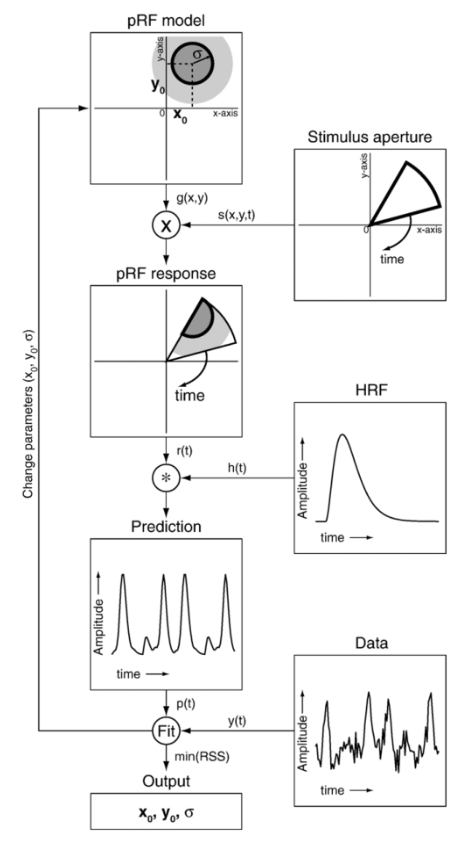
\includegraphics[scale=0.6]{../images/pRF model}
\caption{Diagrama de flujo que describe el procedimiento de estimación del modelo pRF. Tomado de [\cite{dumoulin_population_2008}]}
\label{fig:pRF}
\end{figure}

El ajuste de pRF permite derivar varias descripciones detalladas de los datos obtenidos. Entre ellas se encuentran los mapas tradicionales de excentricidad y ángulo polar, que revelan la disposición espacial y la orientación preferida de los campos receptivos en la población neuronal.


\section{Modelo lineal mixto generalizado}

Los modelos lineales mixtos generalizados (GLMM) son una poderosa clase de modelos estadísticos que combinan las características de los modelos lineales generalizados y los modelos mixtos (modelos con variables predictivas tanto fijas como aleatorias). Manejan una amplia gama de tipos de variables de respuesta y una amplia gama de escenarios en los que las observaciones se han muestreado en algún tipo de grupo en lugar de hacerlo de forma completamente independiente. Si bien no pueden hacerlo todo (un experto a veces puede elegir modelos personalizados para mayor flexibilidad (Bolker et al. 2013), los GLMM son rápidos, potentes, pueden ampliarse para manejar complejidades adicionales, como respuestas infladas a cero, y pueden suelen estar equipados con software disponible en el mercado. Las únicas desventajas reales de los GLMM se deben a su generalidad: (1) algunas recetas estándar para pruebas e inferencias de modelos no se aplican, y (2) es fácil construir modelos plausibles que son demasiado complejos para que sus datos los respalden. Los GLMM todavía son parte de la frontera estadística e incluso los expertos no conocen todas las respuestas sobre cómo usarlos, pero este capítulo intentará brindar soluciones prácticas que le permitan utilizar GLMM con sus datos.

%------------------------------------------

Modelos Lineales Mixtos Generalizados (GLMM): Son extensiones de los modelos lineales generalizados que incorporan términos aleatorios para tener en cuenta la variabilidad no explicada por las variables fijas. Se utilizan para analizar datos cuando hay correlación o agrupación en los datos, como en estudios longitudinales o con múltiples niveles de jerarquía.


\chapter{Materiales y M\'etodos}\label{chapter:materials_and_methods}

Para abordar los objetivos establecidos en la introducción, se emplearon los siguientes materiales y métodos.

\section{Datos}

Se emplearon los datos analizados en el estudio de [\cite{broderick_mapping_2022}], donde se lleva a cabo un experimento con la participación de 12 sujetos. El objetivo principal de este experimento fue explicar la relación existente entre la frecuencia espacial y la excentricidad en la región V1 del cerebro. Este estudio proporciona una valiosa base de datos, compuesta por estimaciones de amplitud de respuesta de las activaciones neurales, medidas a trav\'es de fMRI, a los diferentes estímulos presentados a los sujetos durante el experimento. Además, se obtuvieron las soluciones de los campos receptivos poblacionales (pRF) de cada sujeto.

En esta sección, se brindará una explicación detallada sobre la naturaleza de los datos recopilados en este estudio.

\subsection{Amplitudes de respuesta de la activaci\'on neuronal}

Durante la realización del experimento, se procedió al registro de las respuestas BOLD (Blood Oxygen Level Dependent) de los participantes en respuesta a un conjunto de est\'imulos de rejilla novedosos (Ver Figura \ref{fig:stim}). Estos estímulos comprendieron 48 vectores de frecuencia diferentes, distribuidos en 8 fases distintas (0, $\frac{\pi}{4}$, $\frac{\pi}{2}$, ..., $\frac{7\pi}{4}$). Dichos vectores de frecuencia se clasificaron en cinco categorías: angular, radial, espiral hacia adelante, espiral hacia atrás y mixto. Para los primeros cuatro estímulos, se consideraron 10 posibles combinaciones de pares ($\omega_a$,$\omega_r$), donde $\omega_a$ representa la frecuencia angular y $\omega_r$ la frecuencia radial del estímulo, mientras que el último solo abarcó 8 combinaciones posibles (consultar [\cite{broderick_mapping_2022}] para obtener información más detallada). La frecuencia angular $\omega_a$ es un número entero que especifica el número de ciclos de rejilla por revolución alrededor de la imagen, y la frecuencia radial $\omega_r$ especifica el número de radianes por unidad de aumento en $ln(r)$, con $r$ siendo la excentricidad.

\begin{figure}
	\centering
	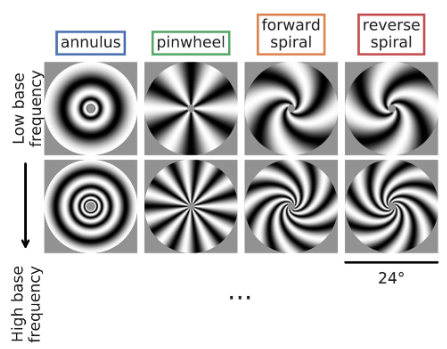
\includegraphics[scale=0.8]{Graphics/stimulus}
	\caption{Ejemplos de est\'imulo angular (annulus), radial (pinwheel), espiral hacia delantes (fordward spiral), espiral hacia atr\'as (reverse spiral), utilizados en [\cite{broderick_mapping_2022}]. Tomado de [\cite{broderick_mapping_2022}].}
	\label{fig:stim}
\end{figure}
Las amplitudes de respuesta a estos estímulos, se estimaron utilizando la caja de herramientas \texttt{GLMdenoise} [\cite{kay_glmdenoise_2013}] en el entorno de programación MATLAB. \texttt{GLMdenoise} es una herramienta diseñada para mejorar la calidad de los datos de fMRI, eliminando artefactos y ruido, lo que facilita una interpretación más precisa de la actividad neuronal. El algoritmo ajusta una función de respuesta hemodinámica (HRF) específica del observador, estimando las amplitudes de respuesta para cada v\'ertice cortical y cada estímulo mediante 100 ejecuciones de bootstrap. La HRF modela la relación temporal entre la actividad neuronal y los cambios en el flujo sanguíneo en el cerebro.

En consecuencia, se obtuvieron 48 respuestas para cada vóxel (una para cada par único de ($\omega_a$,$\omega_r$)), y estas respuestas fueron promediadas a lo largo de las ocho fases presentadas en las pruebas. Además, el algoritmo incorpora tres regresores polinomiales (grados 0 a 2) para capturar la tendencia media de la señal y la deriva lenta, así como regresores de ruido derivados de vóxeles cerebrales que no se ajustan adecuadamente mediante el modelo lineal general. 

Estos datos se pueden encontrar en \href{https://archive.nyu.edu/handle/2451/63344}{NYU Faculty Digital Archive}.

\subsection{Datos de pRF}

Con el objetivo de obtener información precisa sobre la ubicación y tamaño de los pRF en cada sujeto, se llevó a cabo un experimento de retinotopía independiente. 

Los resultados de este mapeo de pRF se integraron con un atlas retinotópico existente desarrollado por [\cite{benson_retinotopic_2012}] utilizando el método de mapa retinotópico bayesiano propuesto por [\cite{benson_human_2018}]. Este enfoque aprovecha la información detallada de la respuesta de los pRF y la estructura de referencia proporcionada por el atlas retinotópico, lo que permite obtener una representación más precisa y confiable de la organización retinotópica en el cerebro de cada sujeto.

Las estimaciones obtenidas mediante el método bayesiano incluyen la excentricidad, el ángulo polar, el tamaño de los pRF y la delimitación de áreas visuales específicas para cada sujeto. Las áreas visuales estimadas abarcan V1, V2, V3, hV4, VO1, VO2, LO1, LO2, TO1, TO2, V3b y V3a.

El método bayesiano se llevó a cabo utilizando la biblioteca \texttt{neuropythy} [\cite{benson_human_2018}] de Python, la cual facilita la manipulación y el análisis de datos neurocientíficos. Los datos estan disponibles en \href{https://openneuro.org/datasets/ds003812/versions/1.1.0}{OpenNeuro}.


\section{Estimaci\'on de per\'iodo preferido}

En el análisis de los datos mencionados, se empleó la modelación propuesta en [\cite{broderick_mapping_2022}] para ajustar una curva de sintonización log-normal unidimensional a las estimaciones de amplitud de respuesta neural de cada voxel, con el objetivo de estimar los valores de período preferido de cada voxel.

La ecuación del modelo utilizada es la siguiente:
\begin{equation}
\hat{\beta}_b(w_l) = A_b \cdot \exp\left(\frac{-(\log_2(w_l) + \log_2(p_b))^2}{2\sigma_b^2}\right)
\end{equation}
donde \(\hat{\beta}_b(w_l)\) representa la respuesta BOLD promedio en el intervalo de excentricidad \(b\) a la frecuencia espacial \(w_l\) (en ciclos por grado). Los parámetros del modelo incluyen \(A_b\), que es la ganancia de respuesta, \(p_b\), el período preferido que se define como el recíproco de la frecuencia espacial máxima y se determina como la moda de la curva de sintonización, y \(\sigma_b\), el ancho de banda medido en octavas.

La frecuencia espacial local de un est\'imulo visual se define como la norma euclidiana del vector de frecuencia ($\omega_a$,$\omega_r$) dividida por la excentricidad  $r$ (\ref{wl}), lo que implica que el período espacial local de los estímulos crece linealmente con la excentricidad [\cite{broderick_mapping_2022}].

\begin{equation}
	w_l(r,\theta) = \dfrac{\sqrt{w_a^2 + w_r^2}}{r} 
	\label{wl}
\end{equation}

Para obtener estimaciones robustas de estos parámetros, se realizaron 100 iteraciones de ajuste por sujeto, por clase de estímulo y por excentricidad utilizando el método de bootstrapping. Este enfoque implicó realizar múltiples ajustes utilizando muestras aleatorias con reemplazo de las 12 ejecuciones de fMRI disponibles (una por cada sujeto).

El método de bootstrapping contribuye a la robustez de los resultados al tener en cuenta la variabilidad natural de las respuestas neuronales a lo largo de múltiples repeticiones del experimento. Así, se logra una caracterización detallada de la respuesta de cada voxel, proporcionando información valiosa sobre la frecuencia espacial preferida para diferentes estímulos visuales y en diversas regiones de la excentricidad en el cerebro.

Los m\'odulos necesarios para aplicar esta estimaci\'on se encuentran en la carpeta src/spf del respositorio adjunto a este documento.

\section{Preprocesamiento de los datos}

En la fase de preprocesamiento de los datos obtenidos en el presente estudio, se llevó a cabo una limpieza para garantizar la confiabilidad y validez de las mediciones. Se tomaron en consideración dos variables particulares de gran importancia en el análisis: la excentricidad y el período preferido de los voxels.

Existen evidencias en la literatura que sugieren que valores extremadamente grandes o pequeños de excentricidad pueden no ser confiables en estudios neurocientíficos \todo{referencias}. Por tanto, se restringi\'o el análisis a v\'oxeles cuya excentricidad se encontraba en un rango entre 1 y 6 unidades. Esta restricción tiene como objetivo mejorar la fiabilidad de las mediciones al excluir valores que podrían introducir sesgos o errores en el análisis.

Para los datos de período preferido de los voxels, se aplicó una transformación logarítmica con el propósito de abordar posibles asimetrías en la distribución y reducir la escala de los datos. Además, se llevó a cabo un filtrado al considerar únicamente aquellos valores cuyo logaritmo era mayor que -6. Esta decisión se basa en la necesidad de excluir valores extremadamente pequeños, que podrían afectar la estabilidad numérica del análisis y no aportarían significativamente a la comprensión de la respuesta neuronal. Esta estrategia también contribuye a manejar posibles datos atípicos que podrían influir negativamente en la interpretación de los resultados.

\section{Modelo lineal mixto}
\label{mlm}
Con el objetivo de validar nuestra hipótesis, la cual postula que la frecuencia espacial preferida de los v\'oxeles en el hemisferio derecho es menor que la preferida en el hemisferio izquierdo, hemos implementado un modelo lineal mixto. Este tipo de modelo es una extensión del modelo lineal clásico y permite considerar tanto efectos fijos como aleatorios en los datos. En esta sección, se detallarán los aspectos fundamentales de la formulación de los modelos diseñados para evaluar cada una de las hipótesis propuestas. Los resultados obtenidos se encuentran en la Figura \ref{fig:mlm_results_pp}.

\subsection{Modelo lineal mixto para frecuencia espacial de est\'imulos visuales}

En la formulación del modelo lineal mixto relacionado con la hip\'otesis, se busca entender la relación entre la frecuencia espacial preferida de los vóxeles y factores como la excentricidad y el hemisferio cerebral. Para ello, utilizando los resultados de [\cite{broderick_mapping_2022}] sobre per\'iodo (inverso de la frecuencia espacial) preferido de los v\'oxeles, se propone el siguiente modelo:

\begin{equation}
	\text{Período Preferido} \sim  \text{Excentricidad} \times \text{Hemisferio} + (1|\text{Sujeto}) + (1|\text{Estímulo})	
	\label{mlm_pp}
\end{equation}
donde:
\begin{itemize}
	\item Período Preferido: Representa la variable dependiente que se desea modelar, y en este contexto, se utiliza como inverso de la frecuencia espacial preferida.
	
	\item Excentricidad y Hemisferio: Son las variables predictoras que se asocian con el período preferido. La interacción entre la excentricidad y el hemisferio permite capturar las posibles influencias conjuntas de estas variables en la respuesta neuronal.
	
	\item (1$|$Subjeto): Este término aleatorio modela la variabilidad entre los diferentes sujetos en el estudio. Cada sujeto puede tener características individuales que contribuyan a la variabilidad en la respuesta neuronal al estímulo visual.

	\item (1$|$Est\'imulo): Representa un término aleatorio para cada estímulo utilizado en el experimento. Diferentes estímulos pueden generar respuestas neurales distintas, y este término captura esa variabilidad entre los estímulos.
	
\end{itemize}

La parte del modelo asociada con la excentricidad y el hemisferio representa los efectos fijos. Estos son los factores que queremos evaluar directamente para comprender cómo afectan al período preferido.

Los términos aleatorios (1$|$sujeto) y (1$|$estímulo) permiten modelar la variabilidad inherente a los datos, considerando las diferencias entre los sujetos y los estímulos. Estos términos aleatorios son esenciales para capturar la heterogeneidad no explicada por los efectos fijos.

Este enfoque proporciona una representación completa y realista de la complejidad de los datos observados en el experimento [\cite{broderick_mapping_2022}].

Se empleó el módulo \texttt{lmer} de R para evaluar este modelo y obtener los coeficientes estimados, errores estándar y valores t de las variables fijas para su análisis.


\subsection{Otros modelos} \label{compare_mlm}

Adicionalmente, se comparan varios modelos lineales mixtos para el período preferido. Este enfoque de comparación entre modelos proporciona perspectivas sobre la relevancia de las variables predictoras en la variabilidad del período preferido. A continuación, se formulan y describen los distintos modelos a comparar:

\begin{itemize}
	\item \textbf{Modelo Nulo:}	\\
	Este modelo considera un intercepto constante como único predictor, sin incluir covariables específicas. La variabilidad entre sujetos y estímulos se captura a través de términos aleatorios. Sirve como punto de referencia para evaluar la mejora en la explicación del período preferido al introducir covariables.
	\begin{equation}
		\text{Período Preferido} \sim 1 + (1|\text{Sujeto}) + (1|\text{Estímulo})	
		\label{m_1}
	\end{equation}

	\item\textbf{Modelo con Excentricidad:}\\
	En este modelo, se agrega la excentricidad como predictor fijo. Se examina cómo la excentricidad se relaciona con el período preferido, considerando la variabilidad entre sujetos y estímulos. Explora si la excentricidad aporta información significativa sobre el período preferido en comparación con el Modelo Nulo.
	\begin{equation}
		\text{Período Preferido} \sim \text{Excentricidad} + (1|\text{Sujeto}) + (1|\text{Estímulo})	
		\label{m_2}
	\end{equation}

	\item \textbf{Modelo con Excentricidad y Hemisferio:}\\
	Este modelo incorpora tanto la excentricidad como el hemisferio como predictores fijos. Se busca evaluar cómo ambas variables influyen en el período preferido, considerando la variabilidad entre sujetos y estímulos. Extiende la exploración al agregar el hemisferio como predictor. Permite evaluar la contribución adicional del hemisferio en la explicación del período preferido.
	\begin{equation}
		\text{Período Preferido} \sim \text{Excentricidad} + \text{Hemisferio} + (1|\text{Sujeto}) + (1|\text{Estímulo})	
		\label{m_3}
	\end{equation}
	
\end{itemize}

%La comparaci\'on de modelos se realiza utilizando el Criterio de Informaci\'on Bayesiana (BIC, por sus siglas en ingl\'es)\todo{citar}, el cual ayuda a evaluar la calidad de diferentes modelos estadísticos para los mismos datos.  
Se calcula el factor de Bayes (BF10) para comparar los modelos. Las comparaciones que se realizan son: el modelo nulo con el modelo con excentricidad, el modelo con excentricidad con el modelo con excentricidad y hemisferio y la \'ultima comparaci\'on es del modelo con excentricidad y hemisferio con el modelo \ref{mlm_pp}, al cual se le adiciona la interacci\'on entre las variables fijas.

En el siguiente cap\'itulo se analizan los resultados pertinentes a estas comparaciones.










\chapter{Resultados}\label{chapter:results}

En este cap\'itulo se presentan los hallazgos clave de nuestro análisis, enfocándose en los resultados relativos a la relación entre el per\'iodo preferido y la excentricidad en diferentes áreas visuales, así como su relevancia en la lateralización hemisférica.

\section{Análisis de la relación entre el tamaño de los pRF y la excentricidad}

\begin{figure}[h]
	\centering
	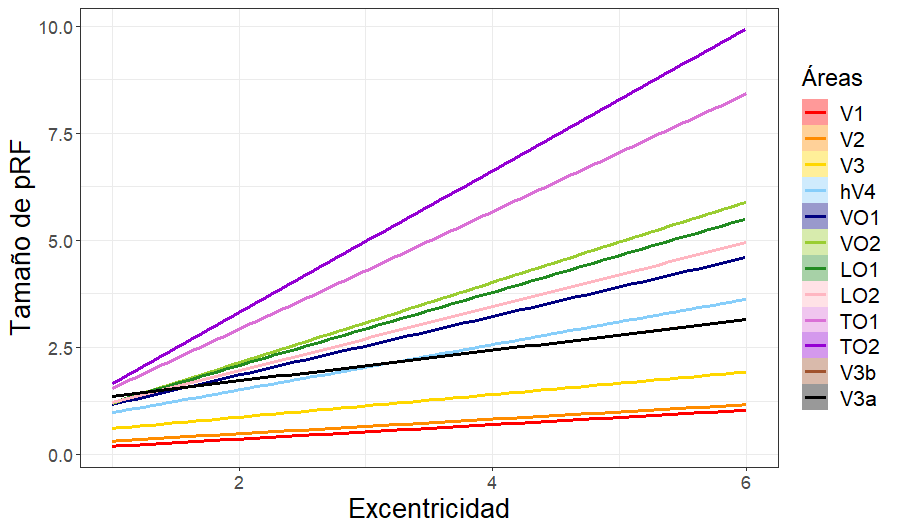
\includegraphics[scale=0.6]{Graphics/size_vs_eccen_bayesian}
	\caption{Gráfico que representa la relación entre el tama\~no de pRF y la excentricidad en las diferentes áreas visuales analizadas.}
	\label{fig:sigma_vs_eccen}
\end{figure}

Aunque no constituye el enfoque principal de este estudio, se llevó a cabo un análisis adicional para examinar la relación entre el tamaño del pRF y la excentricidad en el campo visual. En la Figura \ref{fig:sigma_vs_eccen}, presentamos las rectas de regresión correspondientes a la relaci\'on entre estas variables. Observamos que el tamaño del pRF tiende a incrementarse con la excentricidad, una tendencia que se manifiesta consistentemente a través de las diferentes áreas examinadas. De manera notable, la pendiente de estas rectas de regresión muestra un aumento progresivo al pasar de áreas visuales tempranas, como V1-V3, a áreas de procesamiento visual de nivel superior, tal como TO1. Este hallazgo está en consonancia con investigaciones previas [\cite{wandell_computational_2015}] y refuerza la comprensión de que el tamaño del pRF se expande con la complejidad funcional y jerárquica de las áreas visuales.

\section{Análisis de la relación entre el período preferido y la excentricidad}

En la figura \ref{fig:pp_vs_eccen}, se puede observar que en la mayoría de las áreas visuales analizadas, se cumplen los supuestos de que el período preferido tiende a aumentar con la excentricidad. Sin embargo, es importante destacar que existen variaciones en este patrón.

\begin{figure}[h]
	\centering
	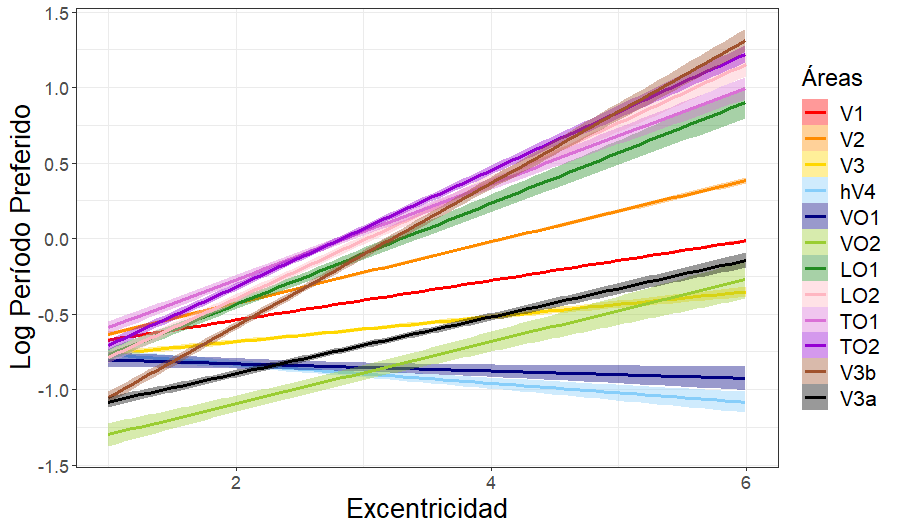
\includegraphics[scale=0.6]{Graphics/pp_vs_eccen}
	\caption{Gráfico que representa la relación entre el logar\'itm del per\'iodo preferido de los v\'oxeles y la excentricidad, en las 12 áreas visuales analizadas.}
	\label{fig:pp_vs_eccen}
\end{figure}

En áreas visuales como hV4 y VO1, se observa una pendiente de crecimiento negativa. Este hallazgo sugiere que, a medida que la excentricidad aumenta, el período preferido tiende a disminuir en lugar de aumentar. Este comportamiento atípico resalta la diversidad de respuestas visuales en diferentes regiones corticales.

Además, en áreas visuales superiores como LO1, LO2, TO1 y TO2,  se evidencia un aumento de la pendiente del período preferido con respecto a la excentricidad, comparado con las áreas visuales tempranas. Esta observación indica que estas áreas específicas muestran un patrón consistente de incremento en el período preferido a medida que nos alejamos del punto central de la visión.

Este análisis proporciona una comprensión más completa de cómo la excentricidad puede modular el período preferido en diversas áreas visuales, destacando la necesidad de considerar la heterogeneidad funcional en la corteza visual.


\section{Resultados del modelo lineal mixto para frecuencias espaciales en función de excentricidad y hemisferio}


En esta secci\'on, se aborda el núcleo central de esta tesis: el análisis del impacto de la frecuencia espacial preferida sobre los hemisferios cerebrales. 

Los resultados obtenidos del modelo lineal mixto \ref{mlm_pp}, aplicado a las frecuencias espaciales de estímulos visuales, se detallan en la Figura \ref{fig:mlm_results_pp}. En esta figura, las filas ilustran las diferentes áreas visuales analizadas mediante el modelo \ref{mlm_pp}, mientras que las columnas, excepto la primera (\'areas), representan las variables fijas con sus respectivos resultados:  estimación de los coeficientes (Coef), error estándar (SE), t-valor (t-val). Adicionalmente, se insert\'o una columna con el factor de Bayes (BF10) con los resultados de la comparaci\'on de cada uno de los modelos propuestos en la secci\'on \ref{mlm}. El BF10 contenido en la columna Excentricidad es resultado de la comparaci\'on del modelo nulo (\ref{m_1}) con el modelo con excentricidad (\ref{m_2}); en la columna Hemisferio de la tabla, se muestra el BF10 de compara los modelos con excentricidad  y con excentricidad y hemisferio (\ref{m_3}) y, en la \'ultima columna se observa el factor BF10 del modelo con excentrididad y hemisferio comparado el modelo \ref{mlm_pp}.


\begin{figure}[h]
	\centering
	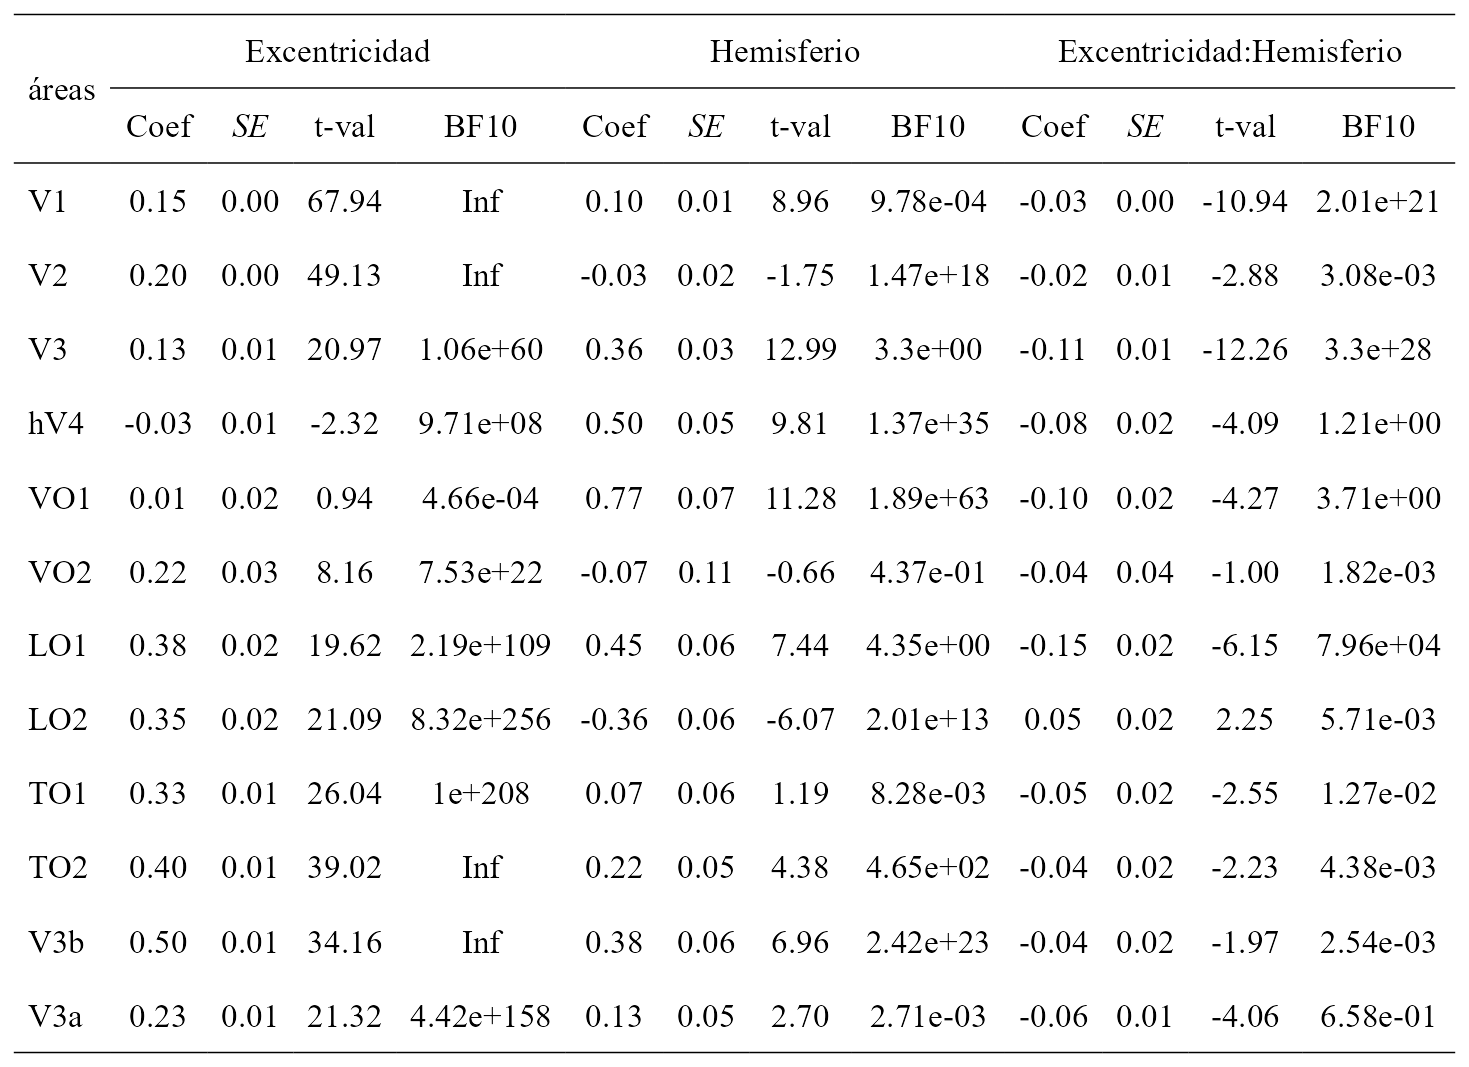
\includegraphics[scale=0.8]{Graphics/table_pp}
	\caption{Tabla que resume los resultados del modelo lineal mixto \ref{mlm_pp} empleado para analizar el per\'iodo preferido de los v\'oxeles en diferentes áreas visuales. Cada fila representa los resultados del modelo para una área visual específica. Para cada variable fija del modelo, la tabla muestra la estimación del coeficiente (Coef), el error estándar (SE) y el valor t (t-val). Además, se incluye el factor de Bayes (BF10) para la comparación entre modelos. El BF10 en la columna 'Excentricidad' corresponde a la comparación entre el modelo \ref{m_1} y \ref{m_2}; en la columna 'Hemisferio', se refiere a la comparación entre el modelo \ref{m_2} y \ref{m_3}; y en la columna 'Excentricidad:Hemisferio', a la comparación entre los modelos \ref{m_3} y \ref{mlm_pp}.}
	\label{fig:mlm_results_pp}
\end{figure}

En el modelo \ref{mlm_pp}, la variable de interés es el periodo preferido, que representa el inverso de la frecuencia espacial. En este modelo, se busca explicar la relación entre el periodo preferido y dos variables independientes: la excentricidad y el hemisferio. Además, se incorporan las diferencias entre sujetos y estímulos para obtener un entendimiento más completo de los factores que influyen en el per\'iodo preferido.

En la Figura \ref{fig:mlm_results_pp}, se aprecia que, con excepción de V01 y hV4, el tamaño del efecto de la excentricidad (Ver Figura \ref{fig:mlm_results_pp}, columna Excentricidad) es mayormente positivo, indicando un aumento en el periodo preferido con la excentricidad. Este hallazgo es respaldado tanto por el valor t como por el factor de Bayes. Además, se observa un patrón consistente de incremento en la magnitud del efecto al pasar de áreas tempranas a aquellas de orden superior, corroborando lo evidenciado en la Figura \ref{fig:pp_vs_eccen}. En el caso de hV4, el coeficiente exhibe un signo negativo y una magnitud inferior en comparación con otras áreas, y es estadísticamente significativo según la prueba t de Student y  el factor de Bayes. Respecto a V01, su coeficiente es notablemente pequeño, y ninguna de las pruebas mencionadas evidencia significancia.

\begin{figure}[h]
	\centering
	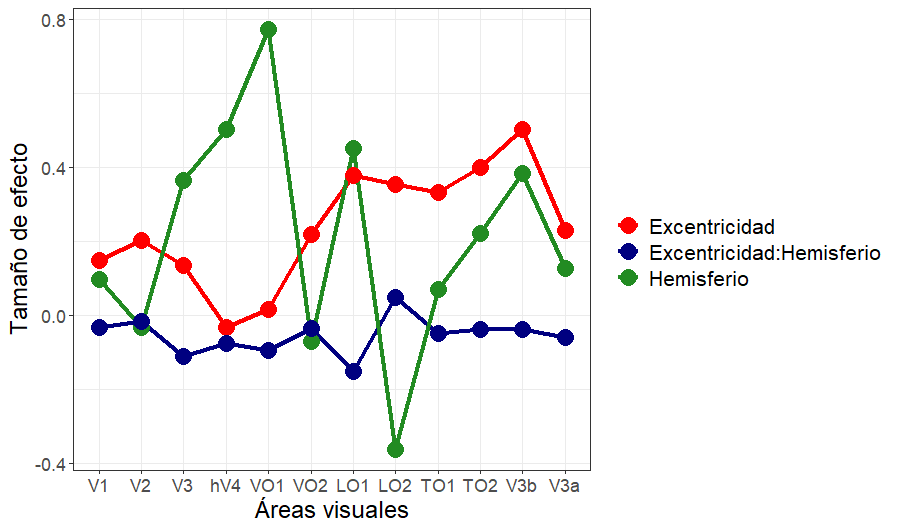
\includegraphics[scale=0.6]{Graphics/effect_size_coef_pp}
	\caption{Representación gráfica de los coeficientes estimados para las variables fijas del modelo lineal mixto \ref{mlm_pp}.}
	\label{fig:coeff}
\end{figure}

Resulta notable que hay un efecto de hemisferio (Ver Figura \ref{fig:mlm_results_pp}, columna Hemisferio) significativo en casi todas las áreas con excepción de V02, pero con coeficientes pequeños en V1, V2, TO1, y V3A . En contraste, las \'areas restantes (V3, hV4, VO1, LO1, LO2, TO2, V3B), presentan coeficientes relativamente grandes (Figura \ref{fig:coeff}), lo cual indica que  el per\'iodo preferido de los v\'ertices corticales en el hemisferio derecho es significativamente mayores que en el izquierdo. Esta diferencia es m\'as pronunciada en las \'areas V01 y hV4 (Ver Figura \ref{fig:hem}). 

Las interacciones entre excentricidad y hemisferio (Ver Figura \ref{fig:mlm_results_pp}, columna Excentricidad:Hemisferio), fueron significativas en varias áreas, pero su magnitud fue relativamente baja en todas las regiones analizadas,

\begin{figure}[h]
	\centering
	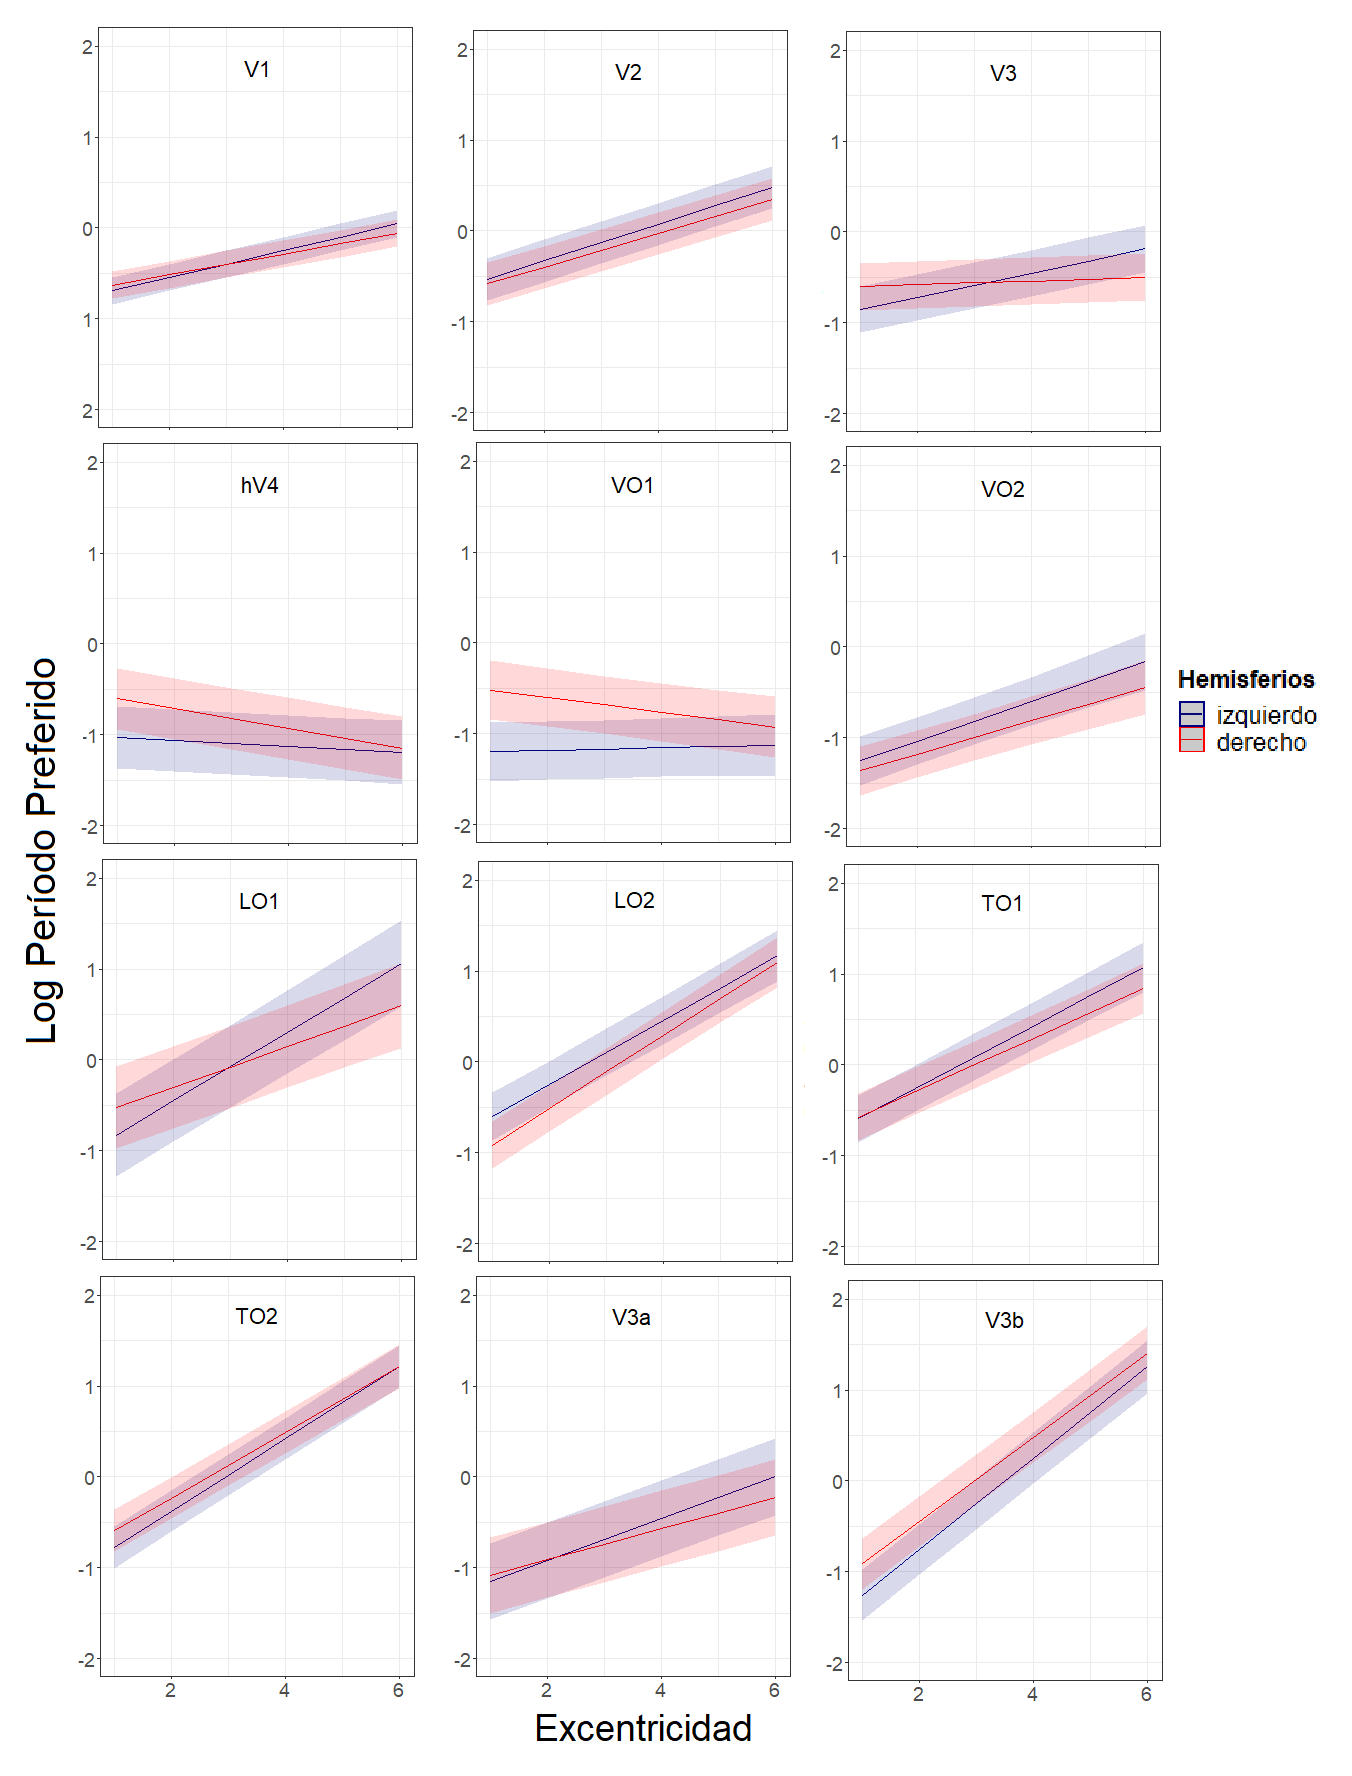
\includegraphics[scale=0.5]{Graphics/compuesto_rois_pp_vs_eccen_hem}
	\caption{Conjunto de gráficas representando la relación entre el logaritmo del per\'iodo preferido de los v\'oxeles y la excentricidad en los dos hemisferios cerebrales, para las 12 áreas visuales analizadas.}
	\label{fig:hem}
\end{figure}














\chapter{Discusi\'on}\label{chapter:discussion}

Se confirma que el tama\~no de pRF de \'areas corticales visuales crece con la excentricidad, y la pendiente de este crecimiento es mayor a medida que se avanza en direcci\'on posterior - anterios en la v\'ia visual. Se confirm\'o Adem\'as que el per\'iodo preferido de v\'ertices corticales en \'areas visuales crece con su excentricidad. Como hllazgo novedoso, se encontr\'o 

Encontramos una relaci\'on directa entre el pe\'riodo preferido y la excentricidad.

Encontramos que en cuatro \'areas visuales (hV4, VO1, TO2, V3b)  el per\'iodo preferido de los v\'ertices corticales era mayor en el hemisferio derecho que en el hemisferio izquierdo. El hemisferio derecho prefiere frecuencias espaciales m\'as bajas que el hemisferio izquierdo. Este efecto no apareci\'o en \'areas visuales primarias (V1-V3) y algunas \'areas de orden superior (ej. LO2).

Tambi\'en se demostr\'o que el tamano de \'areas visuales de los pRF es mayor en el hemisferio derecho 

Esto sugiere que la representaci\'on de las imagenes visuales en algunas \'areas corticales difiere en \'areas superiores.

Muy pocos estudios han examinado la diferencia entre campos receptivos del hemisferio izq-der. Los pocos que lo han hecho se han centrado en \'areas primarias y al igual que nosotros no encuentran diferencias. Los pocos trabajos que han examinado frecuencias espaciales no han comparado hemisferios. Este trabjo es el primer trabajo conocido que halla analiado la diferencia de frecuencias espaciales en ambos hemisferios.

Las estimaciones de pRF parecen m\'as ruidosas que las de preferiencia por sf. Esto se ve en en R2 de las dos variables. Lage y Castellano ha discutido las dificultades que existen en estimar con dificultad el tamono de pRF. 

Los resultados son consistentes con los datos neurosicologicoa neurofisiologico sy neurificos sobre lateral hemis, que coinciden en una ventaja del hemisferio derecho para lo global (sf)y de lo local para hem.izq  esta idea se postulo en la idea de doble filtraje de Robertson sin expecificar posibles circuitos neurales, nuestro analisis sugiere  que este mecanismo podr\'ia surgir de las propiedades discrepantes de los campos receptivos de los dos hemisferios. 

Simulaciones con redes neurales convolucionales prifundas realizadas en CNEURO, que fuereon entrenadas para reconocer letras, (Garea) apoyan esta idea, estas redes se contruyeron con multiples canales que diferian en el tamano y la selectividad en frecuencia de filtros de Gabor como primer paso del procesamiento de imagenes. Los filtros de gabor son el mejor modelo para describir el campo receptivo de celulas visuales o poblaciones neuronales. Cuando se entrena esta redes para discriminar objetos que tienen niveles globales y locales, eliminar los filtros de baja frecuencia impide la percepci\'on de letras locales. Seria interesante construir redes incorporando los parametros medidos en este estudio y hacer una sim mas realista.

La teoria del doble filtraje presupone un ajuste del rango de frecuencias en que se trabaja segun el tipo de estimulo al que entrenta el sujeto. Los sujetos miraban estimulos pequenos centrados en la fovea, es necesario cambiar esto para ver si la preferencia de sf varia. Se sabe que las propiedades de los campos receptivos cambian de acuerdo a la atencion

El estudio ofrece la primera propuesta de un modelo para explicar especializacion hemi de la percepcion glo/local y la primeras clave para la implementacion de RNN




\backmatter

\begin{conclusions}	
	
	En esta investigación, se empleó un modelo lineal mixto para examinar la especialización hemisférica del cerebro en el procesamiento de frecuencias espaciales en la percepción visual.
	
	Los resultados revelaron que tanto el tamaño de los pRFs como el período preferido (inverso de las frecuencias espaciales) de los vértices corticales incrementan con la excentricidad en el campo visual, siendo mayor en \'areas visuales superiores (ej. TO1). A través del análisis de los resultados obtenidos, con el modelo lineal mixto, se observ\'o que el período preferido  de los vóxeles varía entre los hemisferios cerebrales en diversas áreas visuales, lo cual respalda la hipótesis de una lateralización hemisférica. Además, se not\'o que, en las áreas visuales donde se evidencia esta diferencia, el período preferido es más grande en el hemisferio derecho, indicando una inclinación de este hemisferio hacia frecuencias espaciales bajas. Estos hallazgos están en consonancia con datos neurofisiológicos y neuropsicológicos previos [\cite{flevaris_spatial_2016}] sobre la lateralización hemisférica.
	
	Por tanto, se concluye que los resultados de este estudio constituyen aportes significativos al campo de las neurociencias, especialmente en lo que respecta a la comprensión de la selectividad de los hemisferios cerebrales a diferentes frecuencias espaciales en la percepción visual. Los  hallazgos encontrados no solo profundizan nuestro conocimiento del procesamiento visual, sino que también destacan la complejidad y adaptabilidad del cerebro en la interpretación del entorno visual.
	
         
         
\end{conclusions}

\begin{recomendations}
    Recomendaciones
\end{recomendations}

\printbibliography[heading=bibintoc]


\bibliographystyle{plain}

\end{document}